\documentclass[a4paper,12pt]{article}

\title{Exercise 3: Find the Green Box}
\author{Gruppe 6:\\Niels\\Troels\\Mark\\Kristian}

\usepackage[T1]{fontenc}
\usepackage[utf8]{inputenc}
\usepackage[british]{babel}
\usepackage{microtype}

\usepackage{amsmath}

\usepackage{graphicx}

\usepackage[hidelinks]{hyperref}

\setlength{\parskip}{1ex}
\setlength{\parindent}{0pt}
\setlength{\parfillskip}{30pt plus 1 fil}

\begin{document}

\maketitle

\section{Introduction}

For this assignment we have used our webcams and OpenCV 2 to gather pixel data
in addition to the robot sensors.

We split the task into two parts:

\begin{itemize}
\item Locating a green object in a picture
\item Driving
\end{itemize}


\section{Object detection}

To detect a green object in a picture, we developed this algorithm:

\begin{enumerate}
\item Find all green pixels.
\item Remove small groups of green pixels.
\item Find the center of the group of green pixels.
\end{enumerate}


\subsection{Color detection}

OpenCV 2 returns the pixel data in RGB format.  Our program does this:

\begin{enumerate}
\item

Convert all pixels to HSV.

\item

For each pixel:

\begin{enumerate}
\item

Calculate how close the pixel hue is to green.  Green is 120$^{\circ}$.  We use
our own general function for that:

\begin{verbatim}
double closeness_hue(double hue_target, double hue, 
                     double s, double v)
\end{verbatim}

This function returns a value between 0.0 and 1.0.  1.0 is fully green, and 0.0
is the least green, using the distance in the HSV color wheel.

To only focus on really green pixels, the function returns 0.0 for pixels with a
green hue but with a low color value or a low color saturation.

The function also lowers the closeness value of non-close pixels by
exponentiating the closeness value with a constant.

\item Set both R, G, and B for the pixel to the green to the closeness-to-green
value.

\end{enumerate}
\item The picture now contains pixels whose values reflect how green the
original pixels were.
\end{enumerate}


\subsection{Picture denoising}

We are only interested in whether there is a fairly large green box, and where
it is.  To make the rest of our job easier, we would like to remove small groups
of green in the picture, so that we have only one large green object left in the
picture.

We use OpenCV's \texttt{erode} library function to do this.  It will however
also erode any large green object a bit, so we use \texttt{dilate} afterwards to
expand the size of any such large object back to closer to its original size.

At the end of this step, the picture should contain either one large white
rectangle -- if the picture is a large green box -- or just blackish values if
there is no large green box in the picture.


\subsection{Box detection}



\subsection{Test}

We have tested our complete detection algorithm by running it with input from
one of our webcams; see figure~\ref{fig:detect-test}.

\begin{figure}[h]
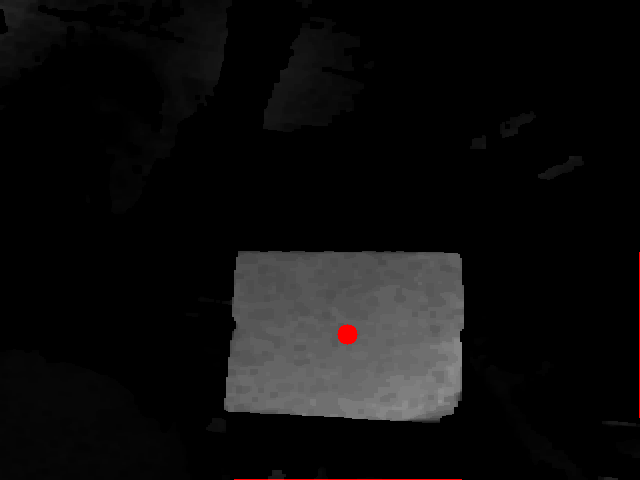
\includegraphics[width=.9\textwidth]{test.png}
\caption{Test of detection algorithm.  The red dot illustrates the center of the
green box.  There is also a red line in the bottom and a red line to the right,
illustrating the length and height of the object, respectively.}
\label{fig:detect-test}
\end{figure}

\section{Driving}




\end{document}
